\documentclass[handout,nooutcomes,noauthor]{ximera}

\graphicspath{  
{./}
{./whoAreYou/}
{./drawingWithTheTurtle/}
{./bisectionMethod/}
{./circles/}
{./anglesAndRightTriangles/}
{./lawOfSines/}
{./lawOfCosines/}
{./plotter/}
{./staircases/}
{./pitch/}
{./qualityControl/}
{./symmetry/}
{./nGonBlock/}
}


%% page layout
\usepackage[cm,headings]{fullpage}
\raggedright
\setlength\headheight{13.6pt}


%% fonts
\usepackage{euler}

\usepackage{FiraMono}
\renewcommand\familydefault{\ttdefault} 
\usepackage[defaultmathsizes]{mathastext}
\usepackage[htt]{hyphenat}

\usepackage[T1]{fontenc}
\usepackage[scaled=1]{FiraSans}

%\usepackage{wedn}
\usepackage{pbsi} %% Answer font


\usepackage{cancel} %% strike through in pitch/pitch.tex


%% \usepackage{ulem} %% 
%% \renewcommand{\ULthickness}{2pt}% changes underline thickness

\tikzset{>=stealth}

\usepackage{adjustbox}

\setcounter{titlenumber}{-1}

%% journal style
\makeatletter
\newcommand\journalstyle{%
  \def\activitystyle{activity-chapter}
  \def\maketitle{%
    \addtocounter{titlenumber}{1}%
                {\flushleft\small\sffamily\bfseries\@pretitle\par\vspace{-1.5em}}%
                {\flushleft\LARGE\sffamily\bfseries\thetitlenumber\hspace{1em}\@title \par }%
                {\vskip .6em\noindent\textit\theabstract\setcounter{question}{0}\setcounter{sectiontitlenumber}{0}}%
                    \par\vspace{2em}
                    \phantomsection\addcontentsline{toc}{section}{\thetitlenumber\hspace{1em}\textbf{\@title}}%
                     }}
\makeatother



%% thm like environments
\let\question\relax
\let\endquestion\relax

\newtheoremstyle{QuestionStyle}{\topsep}{\topsep}%%% space between body and thm
		{}                      %%% Thm body font
		{}                              %%% Indent amount (empty = no indent)
		{\bfseries}            %%% Thm head font
		{)}                              %%% Punctuation after thm head
		{ }                           %%% Space after thm head
		{\thmnumber{#2}\thmnote{ \bfseries(#3)}}%%% Thm head spec
\theoremstyle{QuestionStyle}
\newtheorem{question}{}



\let\freeResponse\relax
\let\endfreeResponse\relax

%% \newtheoremstyle{ResponseStyle}{\topsep}{\topsep}%%% space between body and thm
%% 		{\wedn\bfseries}                      %%% Thm body font
%% 		{}                              %%% Indent amount (empty = no indent)
%% 		{\wedn\bfseries}            %%% Thm head font
%% 		{}                              %%% Punctuation after thm head
%% 		{3ex}                           %%% Space after thm head
%% 		{\underline{\underline{\thmname{#1}}}}%%% Thm head spec
%% \theoremstyle{ResponseStyle}

\usepackage[tikz]{mdframed}
\mdfdefinestyle{ResponseStyle}{leftmargin=1cm,linecolor=black,roundcorner=5pt,
, font=\bsifamily,}%font=\wedn\bfseries\upshape,}


\ifhandout
\NewEnviron{freeResponse}{}
\else
%\newtheorem{freeResponse}{Response:}
\newenvironment{freeResponse}{\begin{mdframed}[style=ResponseStyle]}{\end{mdframed}}
\fi



%% attempting to automate outcomes.

%% \newwrite\outcomefile
%%   \immediate\openout\outcomefile=\jobname.oc
%% \renewcommand{\outcome}[1]{\edef\theoutcomes{\theoutcomes #1~}%
%% \immediate\write\outcomefile{\unexpanded{\outcome}{#1}}}

%% \newcommand{\outcomelist}{\begin{itemize}\theoutcomes\end{itemize}}

%% \NewEnviron{listOutcomes}{\small\sffamily
%% After answering the following questions, students should be able to:
%% \begin{itemize}
%% \BODY
%% \end{itemize}
%% }
\usepackage[tikz]{mdframed}
\mdfdefinestyle{OutcomeStyle}{leftmargin=2cm,rightmargin=2cm,linecolor=black,roundcorner=5pt,
, font=\small\sffamily,}%font=\wedn\bfseries\upshape,}
\newenvironment{listOutcomes}{\begin{mdframed}[style=OutcomeStyle]After answering the following questions, students should be able to:\begin{itemize}}{\end{itemize}\end{mdframed}}



%% my commands

\newcommand{\snap}{{\bfseries\itshape\textsf{Snap!}}}
\newcommand{\flavor}{\link[\snap]{https://snap.berkeley.edu/}}
\newcommand{\mooculus}{\textsf{\textbf{MOOC}\textnormal{\textsf{ULUS}}}}


\usepackage{tkz-euclide}
\tikzstyle geometryDiagrams=[rounded corners=.5pt,ultra thick,color=black]
\colorlet{penColor}{black} % Color of a curve in a plot



\ifhandout\newcommand{\mynewpage}{\newpage}\else\newcommand{\mynewpage}{}\fi


\outcome{Understand the basic idea of the bisection method.}
\outcome{Apply the bisection method to approximate the solution of an equation.}
\outcome{Apply the bisection method to solve a problem where no equation is given.}
\outcome{Describe the bisection method as an algorithm.}


\title{The bisection method}
\author{Bart Snapp}

\begin{document}
\begin{abstract}
  We will use the bisection method to solve triangles.
\end{abstract}
\maketitle

\begin{listOutcomes}
\item{Understand the basic idea of the bisection method.}
\item{Apply the bisection method to approximate the solution of an equation.}
\item{Apply the bisection method to solve a problem where no equation is given.}
\item{Describe the bisection method as an algorithm.}
\end{listOutcomes}
\mynewpage

\begin{question} This question is about the bisection method for approximating solutions to equations.
  \begin{enumerate}
    \item Use the INTERNET to look up the \textbf{bisection
      method}. EXPLAIN the bisection method as you would like to have
      it explained to you.  Use words, pictures, and so on, as
      needed/helpful in your explanation.
  \item USE the bisection method to find a solution (rounded to two
    decimal places) to
  \[
  x^5-x-1=0
  \]
  on the interval $0\le x\le 2$. Display your work with a table:
  \[
  \begin{array}{|c|c|c|c|}\hline
    \text{Attempt} & x & \text{Greater or less than $0$?} \\ \hline\hline
    1 & 0 & less \\ \hline
    2 & 2 & greater  \\ \hline
    3 & ?? & ??  \\ \hline
    \vdots & \vdots & \vdots \\ 
  \end{array}
  \]
  \end{enumerate}
  \begin{freeResponse}
    (a) The \underline{bisection method} helps you find where a curve
    crosses the $x$-axis. The idea is this: If you have a curve and
    you know two $x$-coordinates,
    \begin{itemize}
      \item one where the curve is above the
        $x$-axis and
      \item one where the curve is below the $x$-axis,
    \end{itemize}
    \begin{center}
      \begin{tikzpicture}
        \begin{axis}[
            xmin=-1.2,
            xmax=5.2,
            ymin=-.6,
            ymax=.6,
            axis lines=center,
            xlabel=$x$,
            ylabel=$y$,
            ticks=none,
            every axis y label/.style={at=(current axis.above origin),anchor=south},
            every axis x label/.style={at=(current axis.right of origin),anchor=west},
            %clip=true,
          ]
          \addplot [ultra thick, penColor, smooth] {x^2/20-.5};

          \node[circle,fill,inner sep=2pt] at (axis cs:4,0) {};
          \node[anchor=south east,] at (axis cs:4,.3) {above $x$-axis};

          \draw[dashed] (axis cs: 4,0) -- (axis cs: 4,.3);

          \draw[dashed] (axis cs: 2,0) -- (axis cs: 2,-.3);
          
          \node[circle,fill,inner sep=2pt] at (axis cs:2,0) {};
          \node[anchor=north west,] at (axis cs:2,-.3) {below $x$-axis};
        \end{axis}
      \end{tikzpicture}
    \end{center}
    then you average those $x$-values. This new $x$-value will be
    closer to where the curve crosses the $x$-axis.
    \begin{center}
      \begin{tikzpicture}
        \begin{axis}[
            xmin=-1.2,
            xmax=5.2,
            ymin=-.6,
            ymax=.6,
            axis lines=center,
            xlabel=$x$,
            ylabel=$y$,
            ticks=none,
            every axis y label/.style={at=(current axis.above origin),anchor=south},
            every axis x label/.style={at=(current axis.right of origin),anchor=west},
            %clip=true,
          ]
          \addplot [ultra thick, penColor, smooth] {x^2/20-.5};

          \node[circle,fill,inner sep=2pt] at (axis cs:4,0) {};
          %\node[anchor=south east,] at (axis cs:4,.3) {above $x$-axis};

          \draw[dashed] (axis cs: 4,0) -- (axis cs: 4,.3);

          \draw[dashed] (axis cs: 3,0) -- (axis cs:3,-.05);


          \node[circle,fill,inner sep=2pt,black] at (axis cs:3,0) {};
          \node[] at (axis cs:3,.4) {new point};
          \draw[->] (axis cs: 3,.3) -- (axis cs:3,.1);
          
          \node[circle,fill,inner sep=2pt,black!50!white] at (axis cs:2,0) {};
          \node[] at (axis cs:1,-.1) {old point};

          \draw[->] (axis cs: 3.7,-.4) -- (axis cs:3.95,-.05);

          \draw[->] (axis cs: 3.3,-.4) -- (axis cs:3.05,-.05);
          
          \node[] at (axis cs:3.5,-.5) {average these};
        \end{axis}
      \end{tikzpicture}
    \end{center}


    Repeat this process of averaging the $x$-values that are on
    opposite sides of the $x$-axis. Your $x$-coordinates will get closer
    and closer to where the curve crosses the axis.



    (b) To find an approximate  solution to $x^5-x-1=0$, with the solution rounded to
    two decimal places, write:
    \[
    \begin{array}{|c|c|c|c|}\hline
      \text{Attempt} & \text{x} & \text{Greater or less than $0$?} \\ \hline\hline
      1 & 0 & \text{less} \\ \hline
      2 & 2 & \text{greater}  \\ \hline
      3 & 1 & \text{less}  \\ \hline
      4 & 1.5 & \text{greater}  \\ \hline
      5 & 1.25 & \text{greater}  \\ \hline
      6 & 1.125 & \text{less}  \\ \hline
      7 & 1.1875 & \text{greater}  \\ \hline
      8 & 1.15625 & \text{less}  \\ \hline
      9 & 1.17188 & \text{greater} \\ \hline
      10 & 1.16406 & \text{less} \\ \hline
      11 & 1.16797 & \text{greater} \\ \hline
    \end{array}
    \]
    So we see we have a root at around $x=1.16$, note
    \[
    1.16^5 - 1.16 -1 \approx  -0.06 \approx 0.
    \]
  \end{freeResponse}
\end{question}
\mynewpage

\begin{question}
  Here is a \snap\ script that is supposed to draw a triangle, but the
  last side length is missing:
  
  \adjustbox{valign=t}{
    \begin{tabular}{lp{.7\textwidth}}
 \raisebox{-\height}{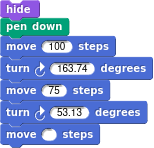
\includegraphics{basicTriangle-script.png}}
      & Clearly EXPLAIN how you can use the bisection method to find
      the FINAL LENGTH  and thus complete the \snap\ script for the
      triangle. Display your work with a table:
          \[
          \begin{array}{|c|c|c|c|}\hline
            \text{Attempt} & \text{Length} & \text{Too short or Too long?} \\ \hline\hline
            1 & ?? & ?? \\ \hline
            2 & ?? & ??  \\ \hline
            \vdots & \vdots & \vdots \\ 
          \end{array}
          \]
  \end{tabular}}
  \begin{freeResponse}
    So, we'll start with a guess for the side length of the triangle,
    say $20$. It's too short. Now, I'll try to get a side length
    long. I picked $50$, and it was too long. Now average them
    together to get $35$. Wow! That's right.  Here is my table
    illustrating this.
    \[
  \begin{array}{|c|c|c|c|}\hline
    \text{Attempt} & \text{Length} & \text{Too short or Too long?} \\ \hline\hline
    1 & 20 & \text{short} \\ \hline
    2 & 50 & \text{long} \\ \hline
    3 & 35 & \text{BINGO!} \\ \hline
  \end{array}
  \]
\end{freeResponse}
\end{question}
\mynewpage

\begin{question}
  The bisection method is an example of a basic \textbf{algorithm}.
  \begin{enumerate}
    \item Find a relevant definition of an \textbf{algorithm}, and state it in
      your own words.
    \item  Give step-by-step instructions for using bisection method to find
  the final side length of a triangle, assuming you know two sides and
  all three angles.
  \end{enumerate}
  \begin{freeResponse}
    \begin{enumerate}
    \item An \underline{algorithm} is a step-by-step description of how
      to solve a problem that can be applied with minimal thought.
    \item Given two sides of a triangle and all of the angles, we can
      find the third side using the bisection method.

    \begin{enumerate}
      \item Find the sum of the two known sides. This is the maximum
        length the third side could be, call it $M$.
      \item Let $0$ be the minimum length the third side could be. Call this number $m$.
      \item\label{ABS:stop} If $M=m$ or $|M-m|< small-number$ we are done, so STOP.
      \item Now, it must be that $M>m$. Average $M$ and $m$ and call it $a$.
      \item Is $a$ the correct length? If so, then we are done, so STOP.
      \item If $a$ is too long, change $M$ to make it equal to $a$.
      \item If $a$ is too short, change $m$ to make it equal to $a$.
      \item Goto step~\ref{ABS:stop}.
    \end{enumerate}
    \end{enumerate}
  \end{freeResponse}
\end{question}



\end{document}
